\tikzstyle{level 1}=[level distance=1.5cm, sibling distance=6cm]
\tikzstyle{level 2}=[level distance=1.5cm, sibling distance=4.0cm]

\tikzstyle{bag} = [text width=4em, text centered]
\tikzstyle{end} = [circle, minimum width=3pt, fill, inner sep=0pt]

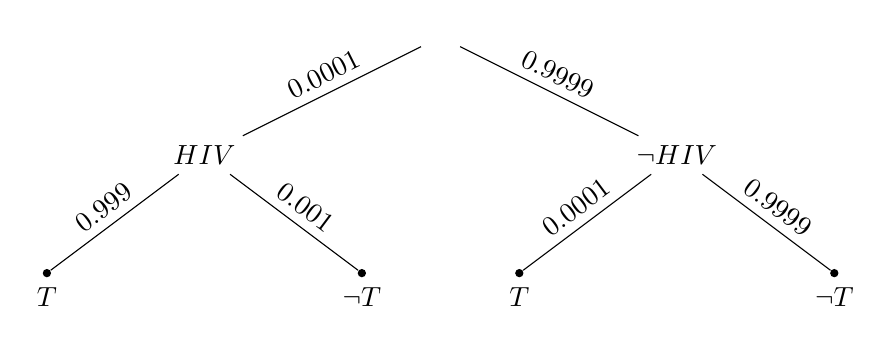
\begin{tikzpicture}[grow=down, sloped]
\node[bag] {}
    child {
        node[bag] {$HIV$}
        child {
            node[end, label=below: {$T$}] {}
            edge from parent
            node[above] {0.999}
        }
        child {
            node[end, label=below: {$\neg T$}] {}
            edge from parent
            node[above] {0.001}
        }
        edge from parent         
        node[above] {0.0001}
    }
    child {
        node[bag] {$\neg HIV$}
        child {
            node[end, label=below: {$T$}] {}
            edge from parent
            node[above] {0.0001}
        }
        child {
            node[end, label=below: {$\neg T$}] {}
            edge from parent
            node[above] {0.9999}
        }
        edge from parent         
        node[above] {0.9999}
    };
\end{tikzpicture}
